%INTRODUCTION
\subsection{Motivation}

...

\subsection{Objectives}

This thesis is part of the ongoing development of the dynamic simulation framework, 
with a focus on extending its capabilities to include small-signal stability analysis and foundational electromagnetic transient (EMT) modeling. 
The work is carried out within the Veragrid environment, where new modules and methodologies are being implemented. 
The main goal is to equip Veragrid with advanced tools for studying the dynamic behavior of power systems, integrating symbolic modeling, numerical routines,
and graphical interfaces for analysis and visualization.

\subsubsection*{General Objectives}

To develop and validate advanced methodologies for dynamic simulation and stability analysis of power systems by incorporating small-signal stability techniques and foundational EMT modeling, fully integrated into the Veragrid environment.

\subsubsection*{Specific Objectives}

\begin{itemize}
    \item To develop the small-signal analysis module for RMS models, including the formulation and linearization of differential-algebraic equations at the operating point,
     the computation of eigenvalues and participation factors from the jacobian matrix, and its integration into Veragrid's graphical interface.
    \item To implement the foundational components for EMT simulation, modeling transmission lines and system elements in the abc domain, applying discretization techniques
     such as the Dommel algorithm and alternatives like the 2S-DIRK method, and validating the EMT solver using benchmark systems compared against commercial tools such as PSCAD.
    \item To extend symbolic system formulation to support custom models and control schemes, improving numerical routines, and ensuring consistent initialization of dynamic studies.
    \item To validate the developed methodologies through case studies, continuously comparing results with commercial tools to ensure model reliability and correctness.
\end{itemize}




\subsection{Scope}

This thesis is part of the ongoing development of Veragrid, a leading software platform for power system planning and simulation. 
The work focuses on improving dynamic simulation tools for modern grids, particularly in the context of small-signal stability and electromagnetic transient (EMT) modeling.
Over a nine-month period—from September 2025 to May 2026—the project aims to build essential components that support symbolic formulation, numerical validation,
and integration with existing simulation environments. 

The first major area of focus is the implementation of small-signal stability analysis using RMS-based state-space models.
This includes the computation of eigenvalues and participation factors, symbolic reduction of system equations,
and integration of these routines into the VeraGrid graphical interface.
The goal is to provide researchers and engineers with intuitive and accurate tools for identifying dominant modes and assessing system stability under varying conditions.

The second area involves the development of a foundational EMT solver in the abc domain. This includes modeling transmission lines and components,
implementing discretization techniques such as the Dommel algorithm and two-stage diagonally implicit Runge-Kutta (2S-DIRK) methods,
and benchmarking solver performance against commercial tools like PSCAD. Although the EMT module is not intended to be exhaustive,
it serves as a proof of concept for future expansion and integration.

All development is conducted in Python, with an emphasis on code quality, symbolic computation, and reproducibility.
The thesis also includes continuous benchmarking and validation using real-world data, including industrial cases.
Technical supervision is provided by the eRoots team, ensuring alignment with architectural standards and long-term project goals.

\subsection{Structure of the document}

This thesis considers all the steps involved in the development process of the RMS small-signal stability analysis and the whole EMT
dynamic simulation, from the mathematical modelling to the software implementation and validation of results.

\begin{itemize}
  \item Chapter \ref{SmallSignal} describes from the theoretical framework to the implementation and benchmarking of the small-signal 
stability analysis in VeraGrid.
  \item Chapter \ref{EMT} describes ...
\end{itemize}

\subsection{State of the art}

things to say:

\textit{The most developed software solutions for EMT simulations
 focusonwaveformdynamicswithandwithoutconverterswitch
ing and include models for very detailed component-level anal
ysis. Examples of software environments are PSCAD, EMTP,
 Simulink, PLECS, among others.}


\subsection{Veragrid}

VeraGrid is a comprehensive software platform for power system planning and simulation, developed to offer both technical accuracy and accessibility. 
It integrates a wide range of analytical and optimization tools, covering everything from traditional steady-state analyses to advanced planning functions 
that address the challenges of modern electrical grids. Its capabilities include conventional studies such as power flow, short-circuit, and contingency analyses, 
as well as linear and non-linear optimization modules used for operational decision-making and long-term investment assessment. Many of these functions are based on 
established industry standards, while others are the result of ongoing research and innovation, designed to push the boundaries of what is possible in open and high-performance 
grid modelling.

\begin{figure}[H]
  \centering
  
\includegraphics[width=0.8\linewidth]{figures/VeraGrid_banner.png}
  \caption{VeraGrid banner. \textit{Source}: VeraGrid documentation \cite{veragrid}.}
  \label{fig:VeraGrid_banner}
\end{figure}

The development of VeraGrid began in 2015 with a clear objective: to create a robust programming library supported by a user-friendly interface. 
This pragmatic vision led to a unique ecosystem where reliability and simplicity coexist with scientific rigour. Over the years, the platform has evolved through a combination 
of commercial projects, academic collaborations, and internal research initiatives, ensuring that its algorithms and methods remain both practical and forward-looking. 
Some of its innovations emerged from the need to address real-world industrial requirements, while others stemmed from curiosity and the exploration of new computational paradigms.

VeraGrid serves a wide audience. For professionals, it provides transparent, efficient, and reproducible tools that enable detailed grid analysis and operational planning. 
For researchers, it represents an open and validated environment capable of integrating experimental algorithms and comparing methodologies. For educators and students, 
it offers a pedagogical platform that connects theoretical concepts with practical, industry-grade implementations. This versatility allows VeraGrid to act as a bridge between 
academia, industry, and future generations of engineers.

Beyond conventional functionalities, VeraGrid includes an extensive set of features designed for modern power systems. 
These include a multi-layered architecture for both usability and computational efficiency; an AC/DC generalized power flow engine that supports hybrid 
grids and converter-based systems; short-circuit and fault analysis modules that incorporate converter control logic; and a suite of optimal power flow, expansion planning, 
and investment analysis tools. The platform also integrates time-series simulation capabilities for renewable energy forecasting, storage operation, and market coupling, 
enabling comprehensive scenario-based studies. 

Thanks to its open-core design, VeraGrid can be easily extended and interfaced with external tools, ensuring interoperability and adaptability to specific project needs. 
It stands not only as a software product but as a complete analytical framework that evolves alongside the energy transition, enabling engineers, researchers, and institutions 
to model, plan, and optimize electrical networks with transparency and scientific depth.

\begin{figure}[H]
  \centering
  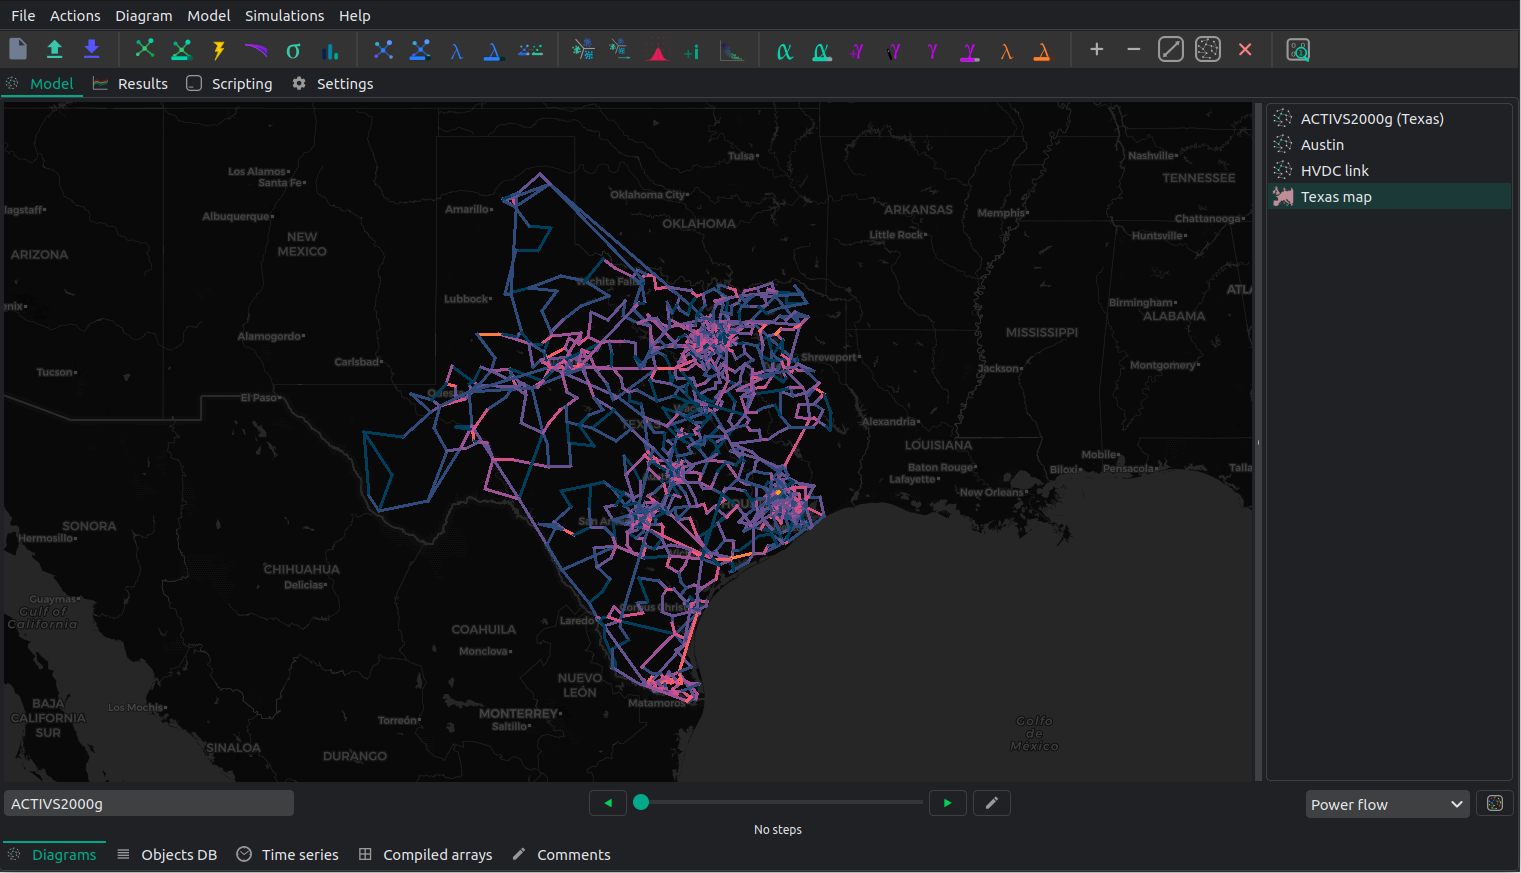
\includegraphics[width=0.8\linewidth]{figures/VeraGrid_main_page.png}
  \caption{VeraGrid main page. \textit{Source}: VeraGrid documentation \cite{veragrid}.}
  \label{fig:VeraGrid_main}
\end{figure}


\newpage